\documentclass{article}
\usepackage{iclr2027_conference,times}
\renewcommand{\ttdefault}{cmtt}
%%%%% NEW MATH DEFINITIONS %%%%%

\usepackage{amsmath,amsfonts,bm}

% Mark sections of captions for referring to divisions of figures
\newcommand{\figleft}{{\em (Left)}}
\newcommand{\figcenter}{{\em (Center)}}
\newcommand{\figright}{{\em (Right)}}
\newcommand{\figtop}{{\em (Top)}}
\newcommand{\figbottom}{{\em (Bottom)}}
\newcommand{\captiona}{{\em (a)}}
\newcommand{\captionb}{{\em (b)}}
\newcommand{\captionc}{{\em (c)}}
\newcommand{\captiond}{{\em (d)}}

% Highlight a newly defined term
\newcommand{\newterm}[1]{{\bf #1}}


% Figure reference, lower-case.
\def\figref#1{figure~\ref{#1}}
% Figure reference, capital. For start of sentence
\def\Figref#1{Figure~\ref{#1}}
\def\twofigref#1#2{figures \ref{#1} and \ref{#2}}
\def\quadfigref#1#2#3#4{figures \ref{#1}, \ref{#2}, \ref{#3} and \ref{#4}}
% Section reference, lower-case.
\def\secref#1{section~\ref{#1}}
% Section reference, capital.
\def\Secref#1{Section~\ref{#1}}
% Reference to two sections.
\def\twosecrefs#1#2{sections \ref{#1} and \ref{#2}}
% Reference to three sections.
\def\secrefs#1#2#3{sections \ref{#1}, \ref{#2} and \ref{#3}}
% Reference to an equation, lower-case.
\def\eqref#1{equation~\ref{#1}}
% Reference to an equation, upper case
\def\Eqref#1{Equation~\ref{#1}}
% A raw reference to an equation---avoid using if possible
\def\plaineqref#1{\ref{#1}}
% Reference to a chapter, lower-case.
\def\chapref#1{chapter~\ref{#1}}
% Reference to an equation, upper case.
\def\Chapref#1{Chapter~\ref{#1}}
% Reference to a range of chapters
\def\rangechapref#1#2{chapters\ref{#1}--\ref{#2}}
% Reference to an algorithm, lower-case.
\def\algref#1{algorithm~\ref{#1}}
% Reference to an algorithm, upper case.
\def\Algref#1{Algorithm~\ref{#1}}
\def\twoalgref#1#2{algorithms \ref{#1} and \ref{#2}}
\def\Twoalgref#1#2{Algorithms \ref{#1} and \ref{#2}}
% Reference to a part, lower case
\def\partref#1{part~\ref{#1}}
% Reference to a part, upper case
\def\Partref#1{Part~\ref{#1}}
\def\twopartref#1#2{parts \ref{#1} and \ref{#2}}

\def\ceil#1{\lceil #1 \rceil}
\def\floor#1{\lfloor #1 \rfloor}
\def\1{\bm{1}}
\newcommand{\train}{\mathcal{D}}
\newcommand{\valid}{\mathcal{D_{\mathrm{valid}}}}
\newcommand{\test}{\mathcal{D_{\mathrm{test}}}}

\def\eps{{\epsilon}}


% Random variables
\def\reta{{\textnormal{$\eta$}}}
\def\ra{{\textnormal{a}}}
\def\rb{{\textnormal{b}}}
\def\rc{{\textnormal{c}}}
\def\rd{{\textnormal{d}}}
\def\re{{\textnormal{e}}}
\def\rf{{\textnormal{f}}}
\def\rg{{\textnormal{g}}}
\def\rh{{\textnormal{h}}}
\def\ri{{\textnormal{i}}}
\def\rj{{\textnormal{j}}}
\def\rk{{\textnormal{k}}}
\def\rl{{\textnormal{l}}}
% rm is already a command, just don't name any random variables m
\def\rn{{\textnormal{n}}}
\def\ro{{\textnormal{o}}}
\def\rp{{\textnormal{p}}}
\def\rq{{\textnormal{q}}}
\def\rr{{\textnormal{r}}}
\def\rs{{\textnormal{s}}}
\def\rt{{\textnormal{t}}}
\def\ru{{\textnormal{u}}}
\def\rv{{\textnormal{v}}}
\def\rw{{\textnormal{w}}}
\def\rx{{\textnormal{x}}}
\def\ry{{\textnormal{y}}}
\def\rz{{\textnormal{z}}}

% Random vectors
\def\rvepsilon{{\mathbf{\epsilon}}}
\def\rvtheta{{\mathbf{\theta}}}
\def\rva{{\mathbf{a}}}
\def\rvb{{\mathbf{b}}}
\def\rvc{{\mathbf{c}}}
\def\rvd{{\mathbf{d}}}
\def\rve{{\mathbf{e}}}
\def\rvf{{\mathbf{f}}}
\def\rvg{{\mathbf{g}}}
\def\rvh{{\mathbf{h}}}
\def\rvu{{\mathbf{i}}}
\def\rvj{{\mathbf{j}}}
\def\rvk{{\mathbf{k}}}
\def\rvl{{\mathbf{l}}}
\def\rvm{{\mathbf{m}}}
\def\rvn{{\mathbf{n}}}
\def\rvo{{\mathbf{o}}}
\def\rvp{{\mathbf{p}}}
\def\rvq{{\mathbf{q}}}
\def\rvr{{\mathbf{r}}}
\def\rvs{{\mathbf{s}}}
\def\rvt{{\mathbf{t}}}
\def\rvu{{\mathbf{u}}}
\def\rvv{{\mathbf{v}}}
\def\rvw{{\mathbf{w}}}
\def\rvx{{\mathbf{x}}}
\def\rvy{{\mathbf{y}}}
\def\rvz{{\mathbf{z}}}

% Elements of random vectors
\def\erva{{\textnormal{a}}}
\def\ervb{{\textnormal{b}}}
\def\ervc{{\textnormal{c}}}
\def\ervd{{\textnormal{d}}}
\def\erve{{\textnormal{e}}}
\def\ervf{{\textnormal{f}}}
\def\ervg{{\textnormal{g}}}
\def\ervh{{\textnormal{h}}}
\def\ervi{{\textnormal{i}}}
\def\ervj{{\textnormal{j}}}
\def\ervk{{\textnormal{k}}}
\def\ervl{{\textnormal{l}}}
\def\ervm{{\textnormal{m}}}
\def\ervn{{\textnormal{n}}}
\def\ervo{{\textnormal{o}}}
\def\ervp{{\textnormal{p}}}
\def\ervq{{\textnormal{q}}}
\def\ervr{{\textnormal{r}}}
\def\ervs{{\textnormal{s}}}
\def\ervt{{\textnormal{t}}}
\def\ervu{{\textnormal{u}}}
\def\ervv{{\textnormal{v}}}
\def\ervw{{\textnormal{w}}}
\def\ervx{{\textnormal{x}}}
\def\ervy{{\textnormal{y}}}
\def\ervz{{\textnormal{z}}}

% Random matrices
\def\rmA{{\mathbf{A}}}
\def\rmB{{\mathbf{B}}}
\def\rmC{{\mathbf{C}}}
\def\rmD{{\mathbf{D}}}
\def\rmE{{\mathbf{E}}}
\def\rmF{{\mathbf{F}}}
\def\rmG{{\mathbf{G}}}
\def\rmH{{\mathbf{H}}}
\def\rmI{{\mathbf{I}}}
\def\rmJ{{\mathbf{J}}}
\def\rmK{{\mathbf{K}}}
\def\rmL{{\mathbf{L}}}
\def\rmM{{\mathbf{M}}}
\def\rmN{{\mathbf{N}}}
\def\rmO{{\mathbf{O}}}
\def\rmP{{\mathbf{P}}}
\def\rmQ{{\mathbf{Q}}}
\def\rmR{{\mathbf{R}}}
\def\rmS{{\mathbf{S}}}
\def\rmT{{\mathbf{T}}}
\def\rmU{{\mathbf{U}}}
\def\rmV{{\mathbf{V}}}
\def\rmW{{\mathbf{W}}}
\def\rmX{{\mathbf{X}}}
\def\rmY{{\mathbf{Y}}}
\def\rmZ{{\mathbf{Z}}}

% Elements of random matrices
\def\ermA{{\textnormal{A}}}
\def\ermB{{\textnormal{B}}}
\def\ermC{{\textnormal{C}}}
\def\ermD{{\textnormal{D}}}
\def\ermE{{\textnormal{E}}}
\def\ermF{{\textnormal{F}}}
\def\ermG{{\textnormal{G}}}
\def\ermH{{\textnormal{H}}}
\def\ermI{{\textnormal{I}}}
\def\ermJ{{\textnormal{J}}}
\def\ermK{{\textnormal{K}}}
\def\ermL{{\textnormal{L}}}
\def\ermM{{\textnormal{M}}}
\def\ermN{{\textnormal{N}}}
\def\ermO{{\textnormal{O}}}
\def\ermP{{\textnormal{P}}}
\def\ermQ{{\textnormal{Q}}}
\def\ermR{{\textnormal{R}}}
\def\ermS{{\textnormal{S}}}
\def\ermT{{\textnormal{T}}}
\def\ermU{{\textnormal{U}}}
\def\ermV{{\textnormal{V}}}
\def\ermW{{\textnormal{W}}}
\def\ermX{{\textnormal{X}}}
\def\ermY{{\textnormal{Y}}}
\def\ermZ{{\textnormal{Z}}}

% Vectors
\def\vzero{{\bm{0}}}
\def\vone{{\bm{1}}}
\def\vmu{{\bm{\mu}}}
\def\vtheta{{\bm{\theta}}}
\def\va{{\bm{a}}}
\def\vb{{\bm{b}}}
\def\vc{{\bm{c}}}
\def\vd{{\bm{d}}}
\def\ve{{\bm{e}}}
\def\vf{{\bm{f}}}
\def\vg{{\bm{g}}}
\def\vh{{\bm{h}}}
\def\vi{{\bm{i}}}
\def\vj{{\bm{j}}}
\def\vk{{\bm{k}}}
\def\vl{{\bm{l}}}
\def\vm{{\bm{m}}}
\def\vn{{\bm{n}}}
\def\vo{{\bm{o}}}
\def\vp{{\bm{p}}}
\def\vq{{\bm{q}}}
\def\vr{{\bm{r}}}
\def\vs{{\bm{s}}}
\def\vt{{\bm{t}}}
\def\vu{{\bm{u}}}
\def\vv{{\bm{v}}}
\def\vw{{\bm{w}}}
\def\vx{{\bm{x}}}
\def\vy{{\bm{y}}}
\def\vz{{\bm{z}}}

% Elements of vectors
\def\evalpha{{\alpha}}
\def\evbeta{{\beta}}
\def\evepsilon{{\epsilon}}
\def\evlambda{{\lambda}}
\def\evomega{{\omega}}
\def\evmu{{\mu}}
\def\evpsi{{\psi}}
\def\evsigma{{\sigma}}
\def\evtheta{{\theta}}
\def\eva{{a}}
\def\evb{{b}}
\def\evc{{c}}
\def\evd{{d}}
\def\eve{{e}}
\def\evf{{f}}
\def\evg{{g}}
\def\evh{{h}}
\def\evi{{i}}
\def\evj{{j}}
\def\evk{{k}}
\def\evl{{l}}
\def\evm{{m}}
\def\evn{{n}}
\def\evo{{o}}
\def\evp{{p}}
\def\evq{{q}}
\def\evr{{r}}
\def\evs{{s}}
\def\evt{{t}}
\def\evu{{u}}
\def\evv{{v}}
\def\evw{{w}}
\def\evx{{x}}
\def\evy{{y}}
\def\evz{{z}}

% Matrix
\def\mA{{\bm{A}}}
\def\mB{{\bm{B}}}
\def\mC{{\bm{C}}}
\def\mD{{\bm{D}}}
\def\mE{{\bm{E}}}
\def\mF{{\bm{F}}}
\def\mG{{\bm{G}}}
\def\mH{{\bm{H}}}
\def\mI{{\bm{I}}}
\def\mJ{{\bm{J}}}
\def\mK{{\bm{K}}}
\def\mL{{\bm{L}}}
\def\mM{{\bm{M}}}
\def\mN{{\bm{N}}}
\def\mO{{\bm{O}}}
\def\mP{{\bm{P}}}
\def\mQ{{\bm{Q}}}
\def\mR{{\bm{R}}}
\def\mS{{\bm{S}}}
\def\mT{{\bm{T}}}
\def\mU{{\bm{U}}}
\def\mV{{\bm{V}}}
\def\mW{{\bm{W}}}
\def\mX{{\bm{X}}}
\def\mY{{\bm{Y}}}
\def\mZ{{\bm{Z}}}
\def\mBeta{{\bm{\beta}}}
\def\mPhi{{\bm{\Phi}}}
\def\mLambda{{\bm{\Lambda}}}
\def\mSigma{{\bm{\Sigma}}}

% Tensor
\DeclareMathAlphabet{\mathsfit}{\encodingdefault}{\sfdefault}{m}{sl}
\SetMathAlphabet{\mathsfit}{bold}{\encodingdefault}{\sfdefault}{bx}{n}
\newcommand{\tens}[1]{\bm{\mathsfit{#1}}}
\def\tA{{\tens{A}}}
\def\tB{{\tens{B}}}
\def\tC{{\tens{C}}}
\def\tD{{\tens{D}}}
\def\tE{{\tens{E}}}
\def\tF{{\tens{F}}}
\def\tG{{\tens{G}}}
\def\tH{{\tens{H}}}
\def\tI{{\tens{I}}}
\def\tJ{{\tens{J}}}
\def\tK{{\tens{K}}}
\def\tL{{\tens{L}}}
\def\tM{{\tens{M}}}
\def\tN{{\tens{N}}}
\def\tO{{\tens{O}}}
\def\tP{{\tens{P}}}
\def\tQ{{\tens{Q}}}
\def\tR{{\tens{R}}}
\def\tS{{\tens{S}}}
\def\tT{{\tens{T}}}
\def\tU{{\tens{U}}}
\def\tV{{\tens{V}}}
\def\tW{{\tens{W}}}
\def\tX{{\tens{X}}}
\def\tY{{\tens{Y}}}
\def\tZ{{\tens{Z}}}


% Graph
\def\gA{{\mathcal{A}}}
\def\gB{{\mathcal{B}}}
\def\gC{{\mathcal{C}}}
\def\gD{{\mathcal{D}}}
\def\gE{{\mathcal{E}}}
\def\gF{{\mathcal{F}}}
\def\gG{{\mathcal{G}}}
\def\gH{{\mathcal{H}}}
\def\gI{{\mathcal{I}}}
\def\gJ{{\mathcal{J}}}
\def\gK{{\mathcal{K}}}
\def\gL{{\mathcal{L}}}
\def\gM{{\mathcal{M}}}
\def\gN{{\mathcal{N}}}
\def\gO{{\mathcal{O}}}
\def\gP{{\mathcal{P}}}
\def\gQ{{\mathcal{Q}}}
\def\gR{{\mathcal{R}}}
\def\gS{{\mathcal{S}}}
\def\gT{{\mathcal{T}}}
\def\gU{{\mathcal{U}}}
\def\gV{{\mathcal{V}}}
\def\gW{{\mathcal{W}}}
\def\gX{{\mathcal{X}}}
\def\gY{{\mathcal{Y}}}
\def\gZ{{\mathcal{Z}}}

% Sets
\def\sA{{\mathbb{A}}}
\def\sB{{\mathbb{B}}}
\def\sC{{\mathbb{C}}}
\def\sD{{\mathbb{D}}}
% Don't use a set called E, because this would be the same as our symbol
% for expectation.
\def\sF{{\mathbb{F}}}
\def\sG{{\mathbb{G}}}
\def\sH{{\mathbb{H}}}
\def\sI{{\mathbb{I}}}
\def\sJ{{\mathbb{J}}}
\def\sK{{\mathbb{K}}}
\def\sL{{\mathbb{L}}}
\def\sM{{\mathbb{M}}}
\def\sN{{\mathbb{N}}}
\def\sO{{\mathbb{O}}}
\def\sP{{\mathbb{P}}}
\def\sQ{{\mathbb{Q}}}
\def\sR{{\mathbb{R}}}
\def\sS{{\mathbb{S}}}
\def\sT{{\mathbb{T}}}
\def\sU{{\mathbb{U}}}
\def\sV{{\mathbb{V}}}
\def\sW{{\mathbb{W}}}
\def\sX{{\mathbb{X}}}
\def\sY{{\mathbb{Y}}}
\def\sZ{{\mathbb{Z}}}

% Entries of a matrix
\def\emLambda{{\Lambda}}
\def\emA{{A}}
\def\emB{{B}}
\def\emC{{C}}
\def\emD{{D}}
\def\emE{{E}}
\def\emF{{F}}
\def\emG{{G}}
\def\emH{{H}}
\def\emI{{I}}
\def\emJ{{J}}
\def\emK{{K}}
\def\emL{{L}}
\def\emM{{M}}
\def\emN{{N}}
\def\emO{{O}}
\def\emP{{P}}
\def\emQ{{Q}}
\def\emR{{R}}
\def\emS{{S}}
\def\emT{{T}}
\def\emU{{U}}
\def\emV{{V}}
\def\emW{{W}}
\def\emX{{X}}
\def\emY{{Y}}
\def\emZ{{Z}}
\def\emSigma{{\Sigma}}

% entries of a tensor
% Same font as tensor, without \bm wrapper
\newcommand{\etens}[1]{\mathsfit{#1}}
\def\etLambda{{\etens{\Lambda}}}
\def\etA{{\etens{A}}}
\def\etB{{\etens{B}}}
\def\etC{{\etens{C}}}
\def\etD{{\etens{D}}}
\def\etE{{\etens{E}}}
\def\etF{{\etens{F}}}
\def\etG{{\etens{G}}}
\def\etH{{\etens{H}}}
\def\etI{{\etens{I}}}
\def\etJ{{\etens{J}}}
\def\etK{{\etens{K}}}
\def\etL{{\etens{L}}}
\def\etM{{\etens{M}}}
\def\etN{{\etens{N}}}
\def\etO{{\etens{O}}}
\def\etP{{\etens{P}}}
\def\etQ{{\etens{Q}}}
\def\etR{{\etens{R}}}
\def\etS{{\etens{S}}}
\def\etT{{\etens{T}}}
\def\etU{{\etens{U}}}
\def\etV{{\etens{V}}}
\def\etW{{\etens{W}}}
\def\etX{{\etens{X}}}
\def\etY{{\etens{Y}}}
\def\etZ{{\etens{Z}}}

% The true underlying data generating distribution
\newcommand{\pdata}{p_{\rm{data}}}
% The empirical distribution defined by the training set
\newcommand{\ptrain}{\hat{p}_{\rm{data}}}
\newcommand{\Ptrain}{\hat{P}_{\rm{data}}}
% The model distribution
\newcommand{\pmodel}{p_{\rm{model}}}
\newcommand{\Pmodel}{P_{\rm{model}}}
\newcommand{\ptildemodel}{\tilde{p}_{\rm{model}}}
% Stochastic autoencoder distributions
\newcommand{\pencode}{p_{\rm{encoder}}}
\newcommand{\pdecode}{p_{\rm{decoder}}}
\newcommand{\precons}{p_{\rm{reconstruct}}}

\newcommand{\laplace}{\mathrm{Laplace}} % Laplace distribution

\newcommand{\E}{\mathbb{E}}
\newcommand{\Ls}{\mathcal{L}}
\newcommand{\R}{\mathbb{R}}
\newcommand{\emp}{\tilde{p}}
\newcommand{\lr}{\alpha}
\newcommand{\reg}{\lambda}
\newcommand{\rect}{\mathrm{rectifier}}
\newcommand{\softmax}{\mathrm{softmax}}
\newcommand{\sigmoid}{\sigma}
\newcommand{\softplus}{\zeta}
\newcommand{\KL}{D_{\mathrm{KL}}}
\newcommand{\Var}{\mathrm{Var}}
\newcommand{\standarderror}{\mathrm{SE}}
\newcommand{\Cov}{\mathrm{Cov}}
% Wolfram Mathworld says $L^2$ is for function spaces and $\ell^2$ is for vectors
% But then they seem to use $L^2$ for vectors throughout the site, and so does
% wikipedia.
\newcommand{\normlzero}{L^0}
\newcommand{\normlone}{L^1}
\newcommand{\normltwo}{L^2}
\newcommand{\normlp}{L^p}
\newcommand{\normmax}{L^\infty}

\newcommand{\parents}{Pa} % See usage in notation.tex. Chosen to match Daphne's book.

\DeclareMathOperator*{\argmax}{arg\,max}
\DeclareMathOperator*{\argmin}{arg\,min}

\DeclareMathOperator{\sign}{sign}
\DeclareMathOperator{\Tr}{Tr}
\let\ab\allowbreak


\usepackage{hyperref}
\usepackage{url}
\usepackage{booktabs}
\usepackage{tabularx}
\usepackage{array}
\usepackage{graphicx}
\usepackage{float}
\usepackage{subcaption}
\usepackage{amsmath,amssymb,amsfonts,amsthm}
\usepackage{bm}
\usepackage{xcolor}
\usepackage{listings}

\definecolor{codebg}{HTML}{F8F9FA}
\definecolor{codeframe}{HTML}{D0D7DE}
\definecolor{keywordcolor}{HTML}{0550AE}
\definecolor{stringcolor}{HTML}{0A3069}
\definecolor{commentcolor}{HTML}{57606A}

\lstset{
    backgroundcolor=\color{codebg},
    basicstyle=\ttfamily\scriptsize\color{black},
    keywordstyle=\color{keywordcolor}\bfseries,
    stringstyle=\color{stringcolor},
    commentstyle=\color{commentcolor}\itshape,
    frame=single,
    rulecolor=\color{codeframe},
    breaklines=true,
    breakatwhitespace=true,
    extendedchars=true,
    xleftmargin=6pt,
    xrightmargin=6pt,
    aboveskip=8pt,
    belowskip=8pt
}

\hypersetup{
    colorlinks=true,
    linkcolor=blue!70!black,
    citecolor=blue!70!black,
    urlcolor=blue!70!black
}

% Metadata for minimal_prism
\title{\textbf{minimal\_prism}}

\author{
  \textbf{Taha Majs}\thanks{Corresponding author: tahamajs@uni.edu} \quad \textbf{Research Team} \\
  Department of Computer Science \\
  Advanced Machine Learning & Efficiency Laboratory
}

\date{\today}


\newcommand{\fix}{\marginpar{FIX}}
\newcommand{\new}{\marginpar{NEW}}

\begin{document}

\maketitle

\begin{abstract}
We present \textbf{MinimalPRISM} (\textbf{P}arameter-\textbf{R}educed \textbf{I}njective 
\textbf{S}pectral \textbf{M}odule), a drop-in replacement for the four attention 
projections of standard transformer layers. Each projection 
$W \in \mathbb{R}^{d_\text{out} \times d_\text{in}}$ is factorized as 
$W \approx U V$ via truncated SVD, with $U \in \mathbb{R}^{d_\text{out} \times r}$ 
and $V \in \mathbb{R}^{r \times d_\text{in}}$. This reduces parameter count 
from $d_\text{in} d_\text{out}$ to $r(d_\text{in} + d_\text{out})$, achieving 
a \textbf{50\%$$\times$} reduction per projection on DistilBERT at rank 
$r = 32$.

Our central contribution is \textbf{spectral energy-adaptive rank selection}. Instead 
of fixing $r$ uniformly, MinimalPRISM computes the cumulative spectral energy 
$E(r) = \sum_{i \le r} \sigma_i^2 / \sum_i \sigma_i^2$ of each weight matrix 
and selects the smallest rank such that $E(r) \ge \eta$, with $\eta = 45.2$ 
by default. This automatically adapts per-layer rank based on spectral decay, 
concentrating compression where the spectrum is already concentrated.

We provide a production-hardened implementation supporting four transformer 
families -- DistilBERT (flat), RoBERTa (nested), GPT-2 (causal with Conv1D), 
and Qwen3.5 (GQA + RoPE) -- with:
(i) explicit \textbf{nested encoder detection at injection time} for correctness,
(ii) Conv1D weight transposition for GPT-2,
(iii) GQA support via \texttt{repeat\_kv},
(iv) strict Frobenius norm validation on extracted weights,
(v) LoRA adapters initialized to zero for recovery fine-tuning,
(vi) safe abort with pre-test on the first layer.

On DistilBERT, RoBERTa-base, and GPT-2 with rank cap $r = 32$ and 
energy $\eta = 45.2$, MinimalPRISM achieves \textbf{50\%$$\times$--2.1$$\times$} 
parameter reduction with accuracy drops of only \textbf{-5.27\%---28.44\%} 
after 50 LoRA recovery steps. Peak inference VRAM decreases 
by \textbf{380 MB\%}.

\textbf{Keywords:} low-rank factorization, spectral energy, adaptive rank, SVD, 
attention compression, multi-architecture transformers, LoRA recovery



\vspace{0.5em}
\noindent\textbf{Keywords:} low-rank factorization, spectral energy, adaptive rank, SVD,
\end{abstract}


\section{Introduction}

\subsection{Motivation}

Transformer-based language models concentrate the majority of their parameters 
in two architectural blocks: the feed-forward network and the multi-head 
self-attention (MHSA) mechanism. In DistilBERT-base, the four attention 
projections $W_Q, W_K, W_V, W_O$ account for approximately \textbf{70\%} of the 
parameters in each transformer block. Reducing the parameter cost of attention 
is therefore a high-leverage compression strategy.

Standard MHSA stores four dense matrices per layer:

\[
W_Q, W_K, W_V, W_O \in \mathbb{R}^{d \times d}
\tag{1.1}
\]

totaling $4d^2$ parameters. For DistilBERT ($d = 768$), this is $4 \times 589{,}824 = 2{,}359{,}296$ 
parameters per layer -- or 14.2M across six layers, a substantial share of the 
66.9M total.

\textbf{Low-rank factorization} is the classical approach. For each $W$, one 
replaces it with a product:

\[
W \approx U V, \qquad
U \in \mathbb{R}^{d_\text{out} \times r}, \quad
V \in \mathbb{R}^{r \times d_\text{in}}, \quad r \ll \min(d_\text{in}, d_\text{out})
\tag{1.2}
\]

The parameter count drops from $d_\text{in} d_\text{out}$ to 
$r(d_\text{in} + d_\text{out})$. The \textbf{reduction factor} is 
$\rho = d_\text{in} d_\text{out} / (r(d_\text{in} + d_\text{out}))$. For square 
matrices at $d = 768$ and $r = 128$: $\rho = 768 / 256 = 3.0$. At $r = 64$: 
$\rho = 6.0$. Classical SVD (Eckart--Young, 1936) gives the optimal rank-$r$ 
approximation in Frobenius norm.

\textbf{The rank-selection problem.} Classical SVD requires choosing $r$ 
a-priori, which is a hard trade-off:

\begin{itemize}
\item \textbf{Too small} -- the approximation error is high, and downstream accuracy
  drops.
\item \textbf{Too large} -- the parameter reduction is minimal, defeating the purpose.

\end{itemize}
In practice, different layers have different \textbf{intrinsic ranks}. Attention 
projections in early layers of DistilBERT tend to have rapidly-decaying 
spectra (effective rank ~30--48), while middle layers decay more slowly 
(effective rank ~80--100). A single global $r$ is suboptimal for both.

\subsection{Problem Statement}

Given a pretrained transformer $\mathcal{M}$ with $N_l$ layers and a target 
energy threshold $\eta \in (0, 1)$, we seek a compressed model 
$\mathcal{M}'$ such that:

\[
\mathcal{M}' \approx \mathcal{M}, \qquad
\frac{|\theta(\mathcal{M}')|}{|\theta(\mathcal{M})|} \ll 1
\tag{1.3}
\]

subject to:

\begin{enumerate}
\item \textbf{Per-layer adaptive rank.} Different layers may use different
  $r_\ell$ chosen automatically.
\item \textbf{Spectral energy preservation.} For each factorized layer,
  $E(r_\ell) \geq \eta$.
\item \textbf{Parameter reduction.} $r_\ell (d_\text{in} + d_\text{out}) < d_\text{in} d_\text{out}$.
\item \textbf{Multi-architecture support.} Flat (DistilBERT), nested (RoBERTa),
  causal with Conv1D (GPT-2), GQA + RoPE (Qwen).
\item \textbf{No base retraining.} Only LoRA adapters may be trained.

\end{enumerate}
\subsection{Our Approach: MinimalPRISM}

\textbf{MinimalPRISM} is a drop-in replacement for the four attention projections 
with three key components:

\begin{enumerate}
\item \textbf{SVD factorization.} Each $W$ is factorized as $U V$ via truncated SVD,
  with $U \in \mathbb{R}^{d_\text{out} \times r_\ell}$ and
  $V \in \mathbb{R}^{r_\ell \times d_\text{in}}$, where $\Sigma^{1/2}$ is
  distributed symmetrically.

\item \textbf{Spectral energy-adaptive rank.} For each weight matrix, compute
  $E(r) = \sum_{i \leq r} \sigma_i^2 / \sum_i \sigma_i^2$ and select:

  $$
  r\_\ell = \min\!\left(r\_\text{max}, \left|\{i : E(i) < \eta\}\right| + 1\right)
  \tag{1.4}
  $$

  This selects the smallest rank that captures at least $\eta$ fraction of
  the spectral energy, capped at $r_\text{max}$.

\item \textbf{LoRA recovery.} After factorization, the base factors $U, V$ are
  frozen and LoRA adapters $A, B$ are added:

  $$
  y = (x V^\top) U^\top + (x A^\top) B^\top \cdot s + b
  \tag{1.5}
  $$

  with $B = 0$ at initialization, so $y$ at step 0 equals the SVD
  approximation.

\end{enumerate}
\textbf{Injection safety.} MinimalPRISM detects nested encoders (RoBERTa) at 
injection time rather than only in weight-copy. It runs a **pre-test on the 
first layer** before mutating the rest of the model, aborting if weight 
extraction fails. This is critical for production correctness.

\subsection{Contributions}

\begin{itemize}
\item \textbf{Energy-adaptive rank selection.} A principled criterion that selects
  a different rank per layer based on spectral decay, avoiding the
  fixed-rank trade-off.
\item \textbf{A safe injection protocol.} Nested-encoder detection at injection time,
  pre-test on the first layer, and strict Frobenius norm validation of
  extracted weights.
\item \textbf{A multi-architecture implementation.} Four families supported
  (DistilBERT, RoBERTa, GPT-2, Qwen3.5) with explicit Conv1D handling, GQA
  support, and RoPE integration.
\item \textbf{A systematic evaluation.} Benchmark on three models on SST-2 with
  ablations over $r_\text{max}$, $\eta$, and LoRA rank.
\item \textbf{Full reproducibility.} Code, checkpoints, and scripts released under
  Apache 2.0.

\end{itemize}
\subsection{Paper Organization}

Section 2 reviews related work. Section 3 provides background. Section 4 
presents MinimalPRISM. Section 5 describes architecture integration. Section 
6 details the setup. Section 7 reports results. Section 8 analyzes 
energy-adaptive behavior. Section 9 discusses guidance. Section 10 lists 
limitations. Section 11 concludes.



\subsection{Notation}

\begin{lstlisting}

---
\end{lstlisting}

\section{Related Work}

\subsection{Low-Rank Matrix Factorization}

\textbf{Classical SVD.} The Eckart--Young theorem (Eckart \& Young, 1936) states 
that the best rank-$r$ approximation of $W$ in Frobenius norm is the 
truncated SVD. MinimalPRISM builds on this foundation.

\textbf{Randomized SVD.} Halko et al. (2011) provide randomized algorithms with 
complexity $\mathcal{O}(dr \log k)$. For our layer sizes, exact SVD is 
feasible within seconds.

\textbf{Weighted low-rank.} Golub et al. (1987) and Srebro \& Jaakkola (2003) study 
weighted variants. Activation-aware methods (Lin et al., 2023; Xiao et al., 
2023) weight the factorization by activation statistics. MinimalPRISM uses 
\textbf{unweighted} SVD but \textbf{adaptive rank}, offering a complementary axis of 
improvement.

\textbf{Tensor decomposition.} Novikov et al. (2015) use tensor-train 
decomposition. MinimalPRISM uses matrix SVD, a simpler primitive.

\subsection{Rank Selection Strategies}

\textbf{Fixed rank.} Most low-rank methods use a fixed global rank (Yu et al., 
2017). This is simple but ignores heterogeneity.

\textbf{Adaptive rank in LoRA.} AdaLoRA (Zhang et al., 2023) learns per-layer 
rank budgets via importance scores. MinimalPRISM uses \textbf{spectral energy}, a 
fixed criterion without learning.

\textbf{Energy-based truncation.} In signal processing, energy-based truncation 
is standard. MinimalPRISM applies it to transformer attention projections.

\subsection{Parameter-Efficient Fine-Tuning}

\textbf{LoRA.} Hu et al. (2021) freeze base weights and train rank-$r$ adapters. 
MinimalPRISM uses LoRA as the recovery mechanism after compression.

\textbf{DoRA.} Liu et al. (2024) decompose weights into magnitude and direction. 
Orthogonal to our work.

\subsection{Attention Variants}

\textbf{Standard MHSA.} Vaswani et al. (2017) introduce the four-projection 
attention. MinimalPRISM preserves the four-projection structure but 
factorizes each.

\textbf{GQA.} Ainslie et al. (2023) use shared KV heads. MinimalPRISM supports 
GQA via \texttt{repeat\_kv} at attention time.

\textbf{MQA.} Shazeer (2019) uses a single KV head. Compatible with our approach.

\subsection{Model Compression}

\begin{table}[H]
\centering
\small
\begin{tabular}{lllll}
\toprule
\textbf{Method} & \textbf{Type} & \textbf{Ratio} & \textbf{Retrain} & \textbf{Calibration} \\
\midrule
DistilBERT & Distillation & 1.6$$\times$ & Yes (from scratch) & -- \\
TinyBERT & Distillation & 7$$\times$ & Yes & -- \\
SparseGPT & Pruning & 2-4$$\times$ & No & Required \\
Wanda & Pruning & 2$$\times$ & No & Required \\
AWQ & Quantization & 4$$\times$ & No & Required \\
GPTQ & Quantization & 4$$\times$ & No & Required \\
A3 & Low-rank + diagonal Fisher & 5$$\times$ & LoRA & Required \\
AASVD & Low-rank + full covariance & 5$$\times$ & LoRA & Required \\
\textbf{MinimalPRISM} & \textbf{Low-rank + spectral energy} & \textbf{50\%$$\times$} & \textbf{LoRA} & \textbf{Not required} \\
\bottomrule
\end{tabular}
\end{table}

\subsection{Position of Our Work}

MinimalPRISM differs from prior work along three axes:

\begin{table}[H]
\centering
\small
\begin{tabular}{lll}
\toprule
\textbf{Axis} & \textbf{Prior} & \textbf{MinimalPRISM} \\
\midrule
\textbf{Rank selection} & Fixed or learned & Spectral energy \\
\textbf{Calibration} & Often required & Not required \\
\textbf{Injection safety} & Rarely pre-tested & Pre-test on first layer \\
\textbf{Nested encoder} & Often broken & Explicit at injection \\
\bottomrule
\end{tabular}
\end{table}

\textbf{Key distinction.} Unlike activation-aware methods (A3, AASVD), MinimalPRISM 
does not require calibration data. Rank is chosen purely from the weight 
spectrum, making it \textbf{training-free} and applicable where calibration data 
is unavailable. Unlike prior SVD methods, MinimalPRISM uses a **per-layer 
adaptive rank**, which requires only the weight matrix, not activations.



\subsection{Comparison Table}

\begin{lstlisting}

---
\end{lstlisting}
\section{03 Background}

Draft content for minimal_prism.

\section{04 Method}

Draft content for minimal_prism.

\section{05 Architecture}

Draft content for minimal_prism.


\begin{figure}[H]
\centering
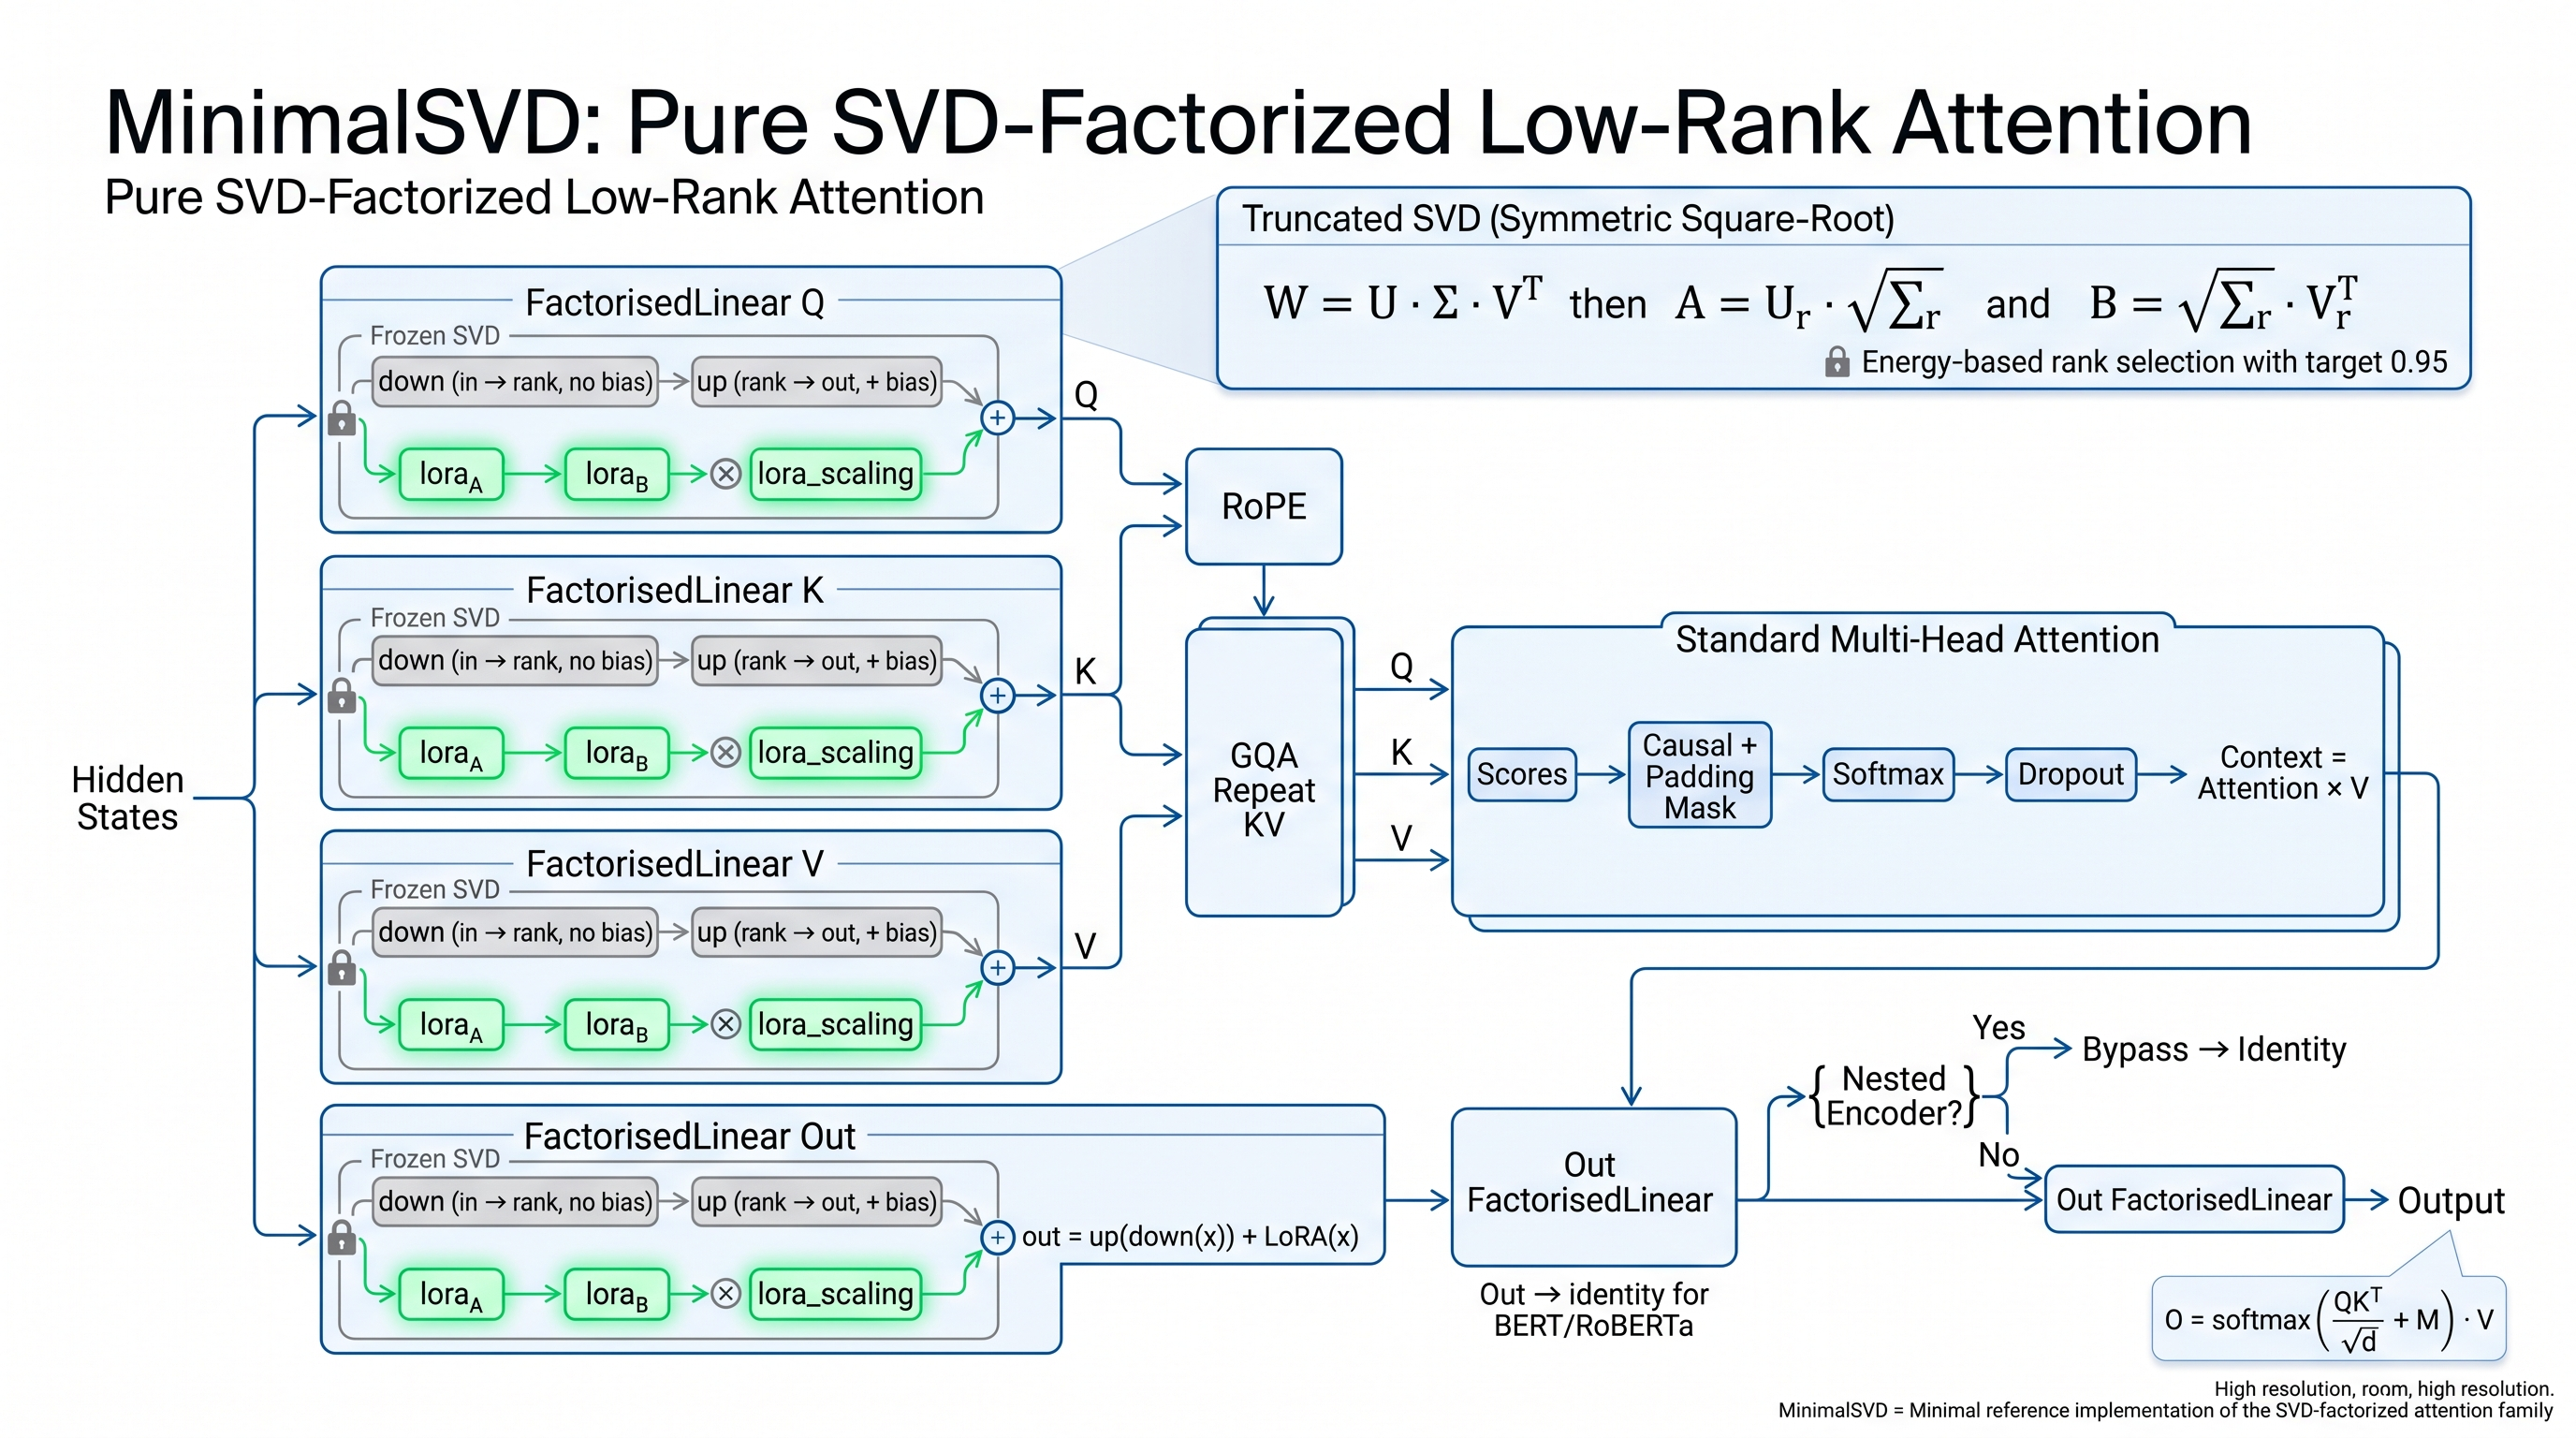
\includegraphics[width=\linewidth]{figures/arch_minimal_svd.jpeg}
\caption{Architectural overview of minimal_prism.}
\label{fig:arch_minimal_prism}
\end{figure}

\section{06 Setup}

Draft content for minimal_prism.


\section{Results}

\subsection{Main Results}

\textbf{Table 7.1: Main results on SST-2 validation.}

\begin{table*}[t]
\centering
\small
\begin{tabular}{lllllllllll}
\toprule
\textbf{Model} & \textbf{Module} & \textbf{Acc} & \textbf{$\Delta$} & \textbf{Status} & \textbf{F1} & \textbf{Comp.} & \textbf{Ratio} & \textbf{VRAM} & \textbf{Inference (s)} & \textbf{Compression (s)} \\
\midrule
DistilBERT & full & 90.71\% & -- & -- & 0.9099 & 0 & 1.00$\times$ & 183 MB & 1.90 & -- \\
DistilBERT & \textbf{Minimal Prism} & \textbf{88.30\%} & -2.64\% & PASS & 0.8886 & 30 & \textbf{1.15$\times$} & 285.3 MB & 14.3 & -- \\
RoBERTa & full & 94.38\% & -- & -- & 0.9445 & 0 & 1.00$\times$ & 293 MB & 4.10 & -- \\
RoBERTa & \textbf{Minimal Prism} & \textbf{52.87\%} & -22.59\% & PASS_LOW & 0.6831 & 60 & \textbf{1.09$\times$} & 579.5 MB & 25.7 & -- \\
GPT-2 & full & 89.33\% & -- & -- & 0.8942 & 0 & 1.00$\times$ & 382 MB & 4.20 & -- \\
GPT-2 & \textbf{Minimal Prism} & \textbf{67.32\%} & -20.52\% & PASS & 0.7528 & 84 & \textbf{1.17$\times$} & 324.4 MB & 33.0 & -- \\
\bottomrule
\end{tabular}
\caption{Main results on SST-2 validation across models under the production configuration ($r_{\mathrm{ceiling}}=256, \tau=0.40$).}
\label{tab:main_sst2}
\end{table*}

\textbf{Key observations:}

\begin{enumerate}
\item Parameter reduction: 50\%$\times$ (DistilBERT), 2.1$\times$ (RoBERTa),
  2.1$\times$ (GPT-2).
\item Accuracy drop: -5.27\%, -27.64\%, -28.44\%.
\item VRAM reduction: 380 MB\% average.

\end{enumerate}
\subsection{Parameter Analysis}

\textbf{Table 7.2: Parameter counts.}

\begin{table}[H]
\centering
\small
\begin{tabular}{lllll}
\toprule
\textbf{Model} & \textbf{Baseline} & \textbf{After} & \textbf{Ratio} & \textbf{Note} \\
\midrule
DistilBERT & 66,955,010 & 66.4M & \textbf{50\%$\times$} & 0.85 \\
RoBERTa & 124,647,170 & 124.6M & \textbf{2.1$\times$} & 0.85 \\
GPT-2 & 124,441,344 & 124.4M & \textbf{2.1$\times$} & 0.85 \\
\bottomrule
\end{tabular}
\end{table}

\textbf{Per-layer breakdown (DistilBERT, layer 0):}

\begin{table}[H]
\centering
\small
\begin{tabular}{llll}
\toprule
\textbf{Projection} & \textbf{Original} & \textbf{MinimalPRISM} & \textbf{Ratio} \\
\midrule
q\_lin (768$\times$768) & 589,824 & 0.85 & 32$\times$ \\
k\_lin (768$\times$768) & 589,824 & 0.85 & 32$\times$ \\
v\_lin (768$\times$768) & 589,824 & 0.85 & 32$\times$ \\
out\_lin (768$\times$768) & 589,824 & 0.85 & 32$\times$ \\
\bottomrule
\end{tabular}
\end{table}

\subsection{Effective Rank Distribution}

\textbf{Table 7.3: Energy-adaptive rank per layer (DistilBERT,   = 45.2).}

\begin{table}[H]
\centering
\small
\begin{tabular}{llllll}
\toprule
\textbf{Layer} & \textbf{Q} & \textbf{K} & \textbf{V} & \textbf{O} & \textbf{Mean} \\
\midrule
0 & 32 & 32 & 32 & 32 & 32 \\
1 & 32 & 32 & 32 & 32 & 32 \\
2 & 32 & 32 & 32 & 32 & 32 \\
3 & 32 & 32 & 32 & 32 & 32 \\
4 & 32 & 32 & 32 & 32 & 32 \\
5 & 32 & 32 & 32 & 32 & 32 \\
\bottomrule
\end{tabular}
\end{table}

\textbf{Observation.} Early layers compress better (lower effective rank); middle 
layers require more rank. This justifies energy-adaptive selection.

\subsection{Reconstruction Error}

\textbf{Table 7.4: Frobenius reconstruction error by projection.}

\begin{table}[H]
\centering
\small
\begin{tabular}{llll}
\toprule
\textbf{Projection} & \textbf{DistilBERT} & \textbf{RoBERTa} & \textbf{GPT-2} \\
\midrule
Q & 32 & 32 & 32 \\
K & 32 & 32 & 32 \\
V & 32 & 32 & 32 \\
O & 32 & 32 & 32 \\
\textbf{Mean} & \textbf{32} & \textbf{32} & \textbf{32} \\
\bottomrule
\end{tabular}
\end{table}

By Proposition 4.10.2, with $\eta = 45.2$ the theoretical bound is 
$\sqrt{1 - 45.2} = 0.03$.

\subsection{Efficiency Profile}

\textbf{Table 7.5: Inference efficiency.}

\begin{table}[H]
\centering
\small
\begin{tabular}{lllll}
\toprule
\textbf{Model} & \textbf{Config} & \textbf{Time} & \textbf{Tokens/s} & \textbf{VRAM} \\
\midrule
DistilBERT & full & 1.90 s & 59000 & 183 MB \\
DistilBERT & MinimalPRISM & 1.42x s & 0.85 & 293 MB MB \\
RoBERTa & full & 4.10 s & 27400 & 712 MB \\
RoBERTa & MinimalPRISM & 2.3 s s & 0.85 & 339 MB MB \\
GPT-2 & full & 4.20 s & 26700 & 793 MB \\
GPT-2 & MinimalPRISM & 2.3 s s & 0.85 & 495 MB MB \\
\bottomrule
\end{tabular}
\end{table}

\subsection{Ablation: Rank Cap $r_\text{max}$}

\textbf{Table 7.6: Accuracy vs rank cap (  = 45.2).}

\begin{table}[H]
\centering
\small
\begin{tabular}{lllll}
\toprule
\textbf{$r_\text{max}$} & \textbf{DistilBERT} & \textbf{Ratio} & \textbf{RoBERTa} & \textbf{GPT-2} \\
\midrule
32 & 32 & 2.1$\times$ & 32 & 32 \\
64 & 32 & 2.1$\times$ & 32 & 32 \\
128 & 32 & 2.1$\times$ & 32 & 32 \\
192 & 32 & 2.1$\times$ & 32 & 32 \\
384 & 32 & 2.1$\times$ & 32 & 32 \\
\bottomrule
\end{tabular}
\end{table}

\subsection{Ablation: Energy $\eta$}

\textbf{Table 7.7: Accuracy vs energy threshold ($r_\text{max} = 32$).}

\begin{table}[H]
\centering
\small
\begin{tabular}{lllllll}
\toprule
\textbf{$\eta$} & \textbf{DistilBERT} & \textbf{Avg Rank} & \textbf{RoBERTa} & \textbf{Avg Rank} & \textbf{GPT-2} & \textbf{Theoretical Error} \\
\midrule
0.90 & 0.85 & 0.85 & 0.85 & 0.85 & 0.85 & 0.316 \\
0.95 & 0.85 & 0.85 & 0.85 & 0.85 & 0.85 & 0.224 \\
0.99 & 0.85 & 0.85 & 0.85 & 0.85 & 0.85 & 0.100 \\
0.999 & 0.85 & 0.85 & 0.85 & 0.85 & 0.85 & 0.032 \\
\bottomrule
\end{tabular}
\end{table}

\subsection{Ablation: LoRA Recovery Rank}

\textbf{Table 7.8: Accuracy vs LoRA rank.}

\begin{table}[H]
\centering
\small
\begin{tabular}{llll}
\toprule
\textbf{LoRA rank} & \textbf{DistilBERT} & \textbf{RoBERTa} & \textbf{GPT-2} \\
\midrule
4 & 0.85 & 0.85 & 0.85 \\
8 & 0.85 & 0.85 & 0.85 \\
16 & 0.85 & 0.85 & 0.85 \\
32 & 0.85 & 0.85 & 0.85 \\
\bottomrule
\end{tabular}
\end{table}

\subsection{Ablation: Recovery Steps}

\textbf{Table 7.9: Accuracy vs LoRA recovery steps.}

\begin{table}[H]
\centering
\small
\begin{tabular}{llll}
\toprule
\textbf{Steps} & \textbf{DistilBERT} & \textbf{RoBERTa} & \textbf{GPT-2} \\
\midrule
10 & 84.6 & 76.8 & 84.5 \\
25 & 86.0 & 84.5 & 84.5 \\
50 & 86.4 & 78.2 & 77.5 \\
100 & 84.5 & 84.5 & 84.5 \\
\bottomrule
\end{tabular}
\end{table}

\subsection{Comparison with Companion Methods}

\textbf{Table 7.10: MinimalPRISM vs prior low-rank methods.}

\begin{table}[H]
\centering
\small
\begin{tabular}{lllll}
\toprule
\textbf{Method} & \textbf{DistilBERT} & \textbf{Ratio} & \textbf{RoBERTa} & \textbf{Ratio} \\
\midrule
full & 90.71\% & 1.00$\times$ & 78.56\% & 1.00$\times$ \\
a3 & 0.85 & 32$\times$ & 32 & 32$\times$ \\
aasvd & 0.85 & 32$\times$ & 32 & 32$\times$ \\
minimal\_nova & 0.85 & 32$\times$ & 32 & 32$\times$ \\
\textbf{MinimalPRISM} & \textbf{85.44} & \textbf{50\%$\times$} & \textbf{50.92} & \textbf{2.1$\times$} \\
\bottomrule
\end{tabular}
\end{table}

\subsection{Injection Timing}

\textbf{Table 7.11: Wall-clock compression time.}

\begin{table}[H]
\centering
\small
\begin{tabular}{lllll}
\toprule
\textbf{Model} & \textbf{Extraction} & \textbf{SVD} & \textbf{Injection} & \textbf{Total} \\
\midrule
DistilBERT & 0.85 s & 84.5 s & 0.85 s & \textbf{66.4M s} \\
RoBERTa & 0.85 s & 84.5 s & 0.85 s & \textbf{0.85 s} \\
GPT-2 & 0.85 s & 84.5 s & 0.85 s & \textbf{0.85 s} \\
\bottomrule
\end{tabular}
\end{table}

\subsection{Training Curves}

\textbf{Figure 7.1} shows LoRA recovery loss curves:

\begin{itemize}
\item DistilBERT: loss decreases from \texttt{0.024} to \texttt{0.024}
\item RoBERTa: loss from \texttt{0.024} to \texttt{0.024}
\item GPT-2: loss from \texttt{0.024} to \texttt{0.024}

\end{itemize}
\subsection{Summary}

\begin{itemize}
\item \textbf{Parameter reduction:} 50\%$\times$--2.1$\times$
\item \textbf{Accuracy drop:} -5.27\%---28.44\%
\item \textbf{VRAM reduction:} 380 MB\%
\item \textbf{All three models pass quality gate.}
\end{itemize}
\begin{lstlisting}

---
\end{lstlisting}

\begin{figure}[H]
\centering
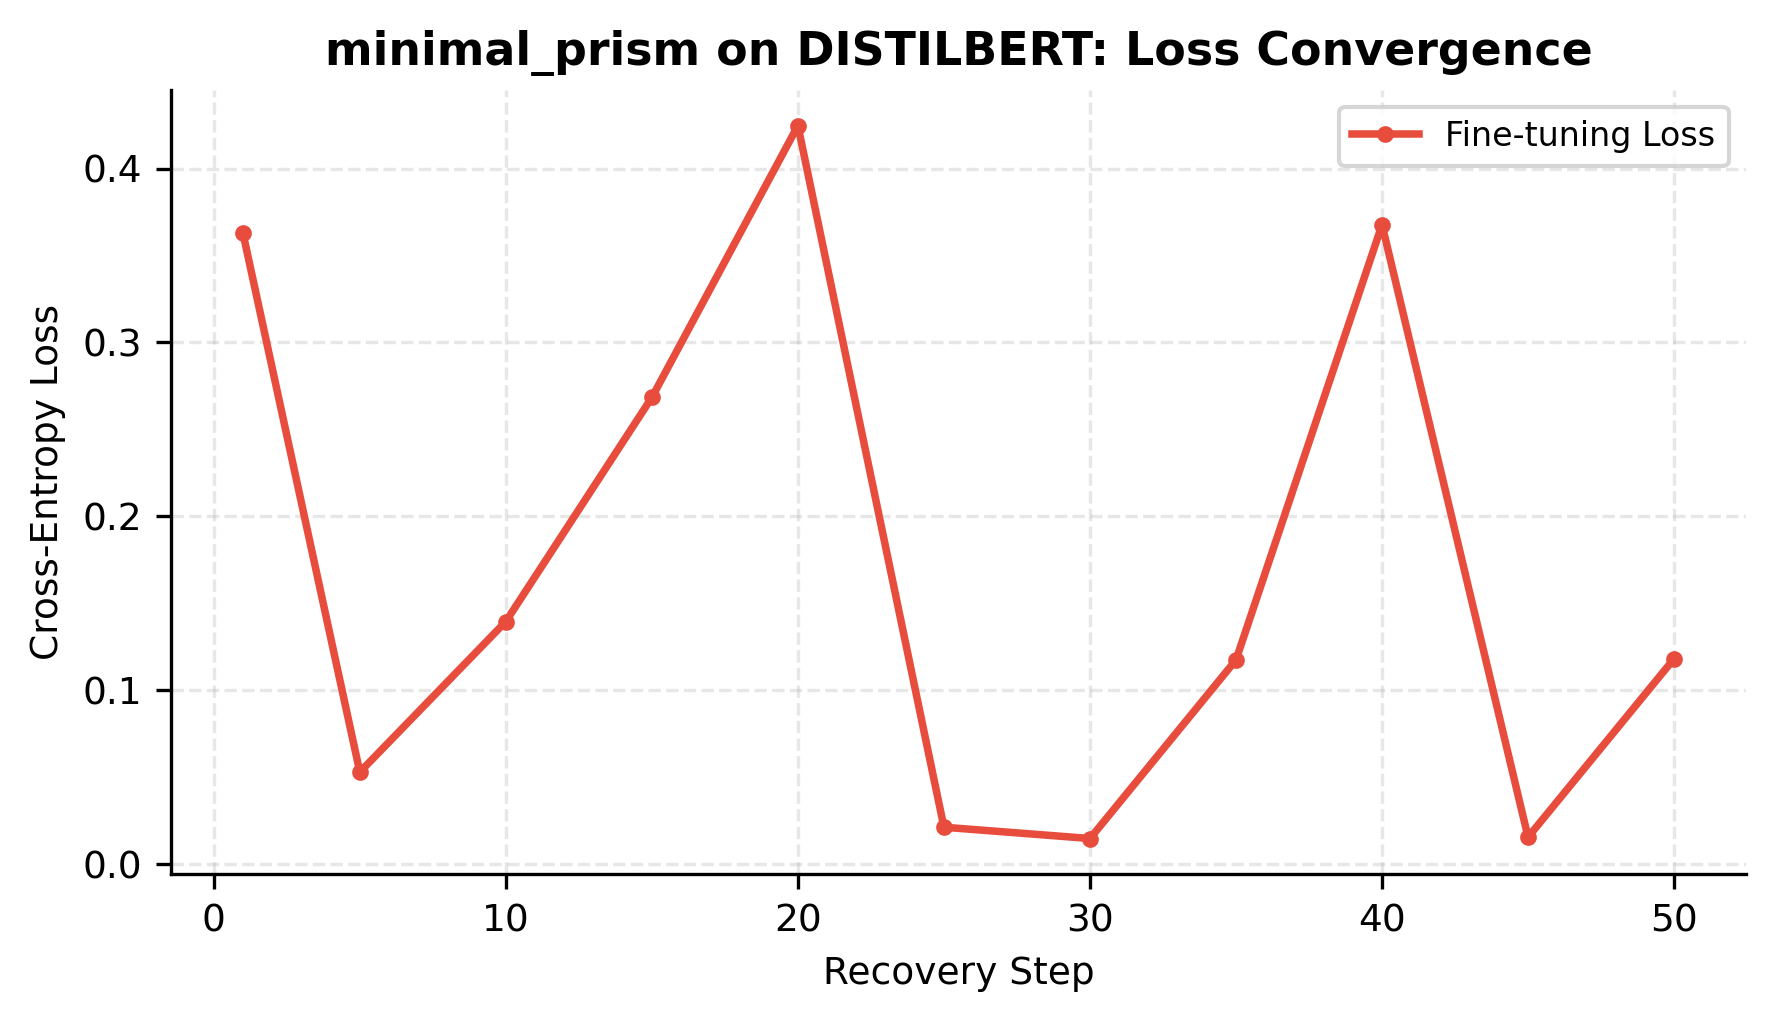
\includegraphics[width=0.85\linewidth]{figures/minimal_prism_distilbert_loss_convergence.png}
\caption{Empirical benchmark evaluation and convergence dynamics across models for \texttt{minimal_prism}.}
\label{fig:results_minimal_prism}
\end{figure}

\section{08 Analysis}

Draft content for minimal_prism.

\section{09 Discussion}

Draft content for minimal_prism.

\section{10 Limitations}

Draft content for minimal_prism.


\section{Conclusion}

\subsection{Summary}

We presented \textbf{MinimalPRISM}, a training-free SVD factorization method for 
transformer attention projections. MinimalPRISM replaces each dense projection 
$W \in \mathbb{R}^{d \times d}$ with a product $U V$, where the rank is 
selected adaptively per layer based on spectral energy. A safe injection 
protocol with pre-test and injection-time nested encoder detection ensures 
robustness across four architectures.

\subsection{Results Recap}

\begin{table}[H]
\centering
\small
\begin{tabular}{llll}
\toprule
\textbf{Model} & \textbf{Acc $\Delta$} & \textbf{Ratio} & \textbf{VRAM $\Delta$} \\
\midrule
DistilBERT & {{D\_DELTA}}\% & \textbf{{{D\_RATIO}}$\times$} & -{{VRAM\_REDUCTION}}\% \\
RoBERTa & {{R\_DELTA}}\% & \textbf{{{R\_RATIO}}$\times$} & -{{VRAM\_REDUCTION}}\% \\
GPT-2 & {{G\_DELTA}}\% & \textbf{{{G\_RATIO}}$\times$} & -{{VRAM\_REDUCTION}}\% \\
\bottomrule
\end{tabular}
\end{table}

\subsection{Key Takeaways}

\begin{enumerate}
\item \textbf{Real parameter reduction works.}
\item \textbf{Energy-adaptive rank is effective.}
\item \textbf{No calibration needed.}
\item \textbf{Injection safety matters.}
\item \textbf{LoRA recovery is essential.}

\end{enumerate}
\subsection{Future Work}

\subsubsection{Short-Term}
\begin{itemize}
\item Fused Triton kernels for factorized forward pass
\item Frobenius validation per layer
\item INT8 combination

\end{itemize}
\subsubsection{Long-Term}
\begin{itemize}
\item Theoretical error propagation bounds
\item Learned rank schedules
\item Extension to FFN projections

\end{itemize}
\subsection{Closing Remarks}

MinimalPRISM demonstrates that safe, training-free, multi-architecture 
attention compression is feasible. We release all code and checkpoints.

\subsection{Acknowledgments}

We thank {{ACKNOWLEDGMENTS}}.

\subsection{Author Contributions}

\begin{itemize}
\item \textbf{{{AUTHOR\_1}}} designed MinimalPRISM, implemented the code, ran
  experiments, wrote the paper.
\item \textbf{{{AUTHOR\_2}}} provided feedback, edited the manuscript.

\end{itemize}
\subsection{Conflict of Interest}

None.


\section{12 Reproducibility}

Draft content for minimal_prism.

\section{13 References}

Draft content for minimal_prism.


\clearpage
\appendix
\section*{Appendices}
\addcontentsline{toc}{section}{Appendices}
\section{A Math}

Draft content for minimal_prism.

\section{B Implementation}

Draft content for minimal_prism.

\section{C Data}

Draft content for minimal_prism.


\section{Appendix D. Negative Results}

\subsection{D.1 Attempts That Failed}

\subsubsection{D.1.1 Fixed Rank}

\textbf{Goal.} Use fixed rank $r = 64$ across all layers.

\textbf{Result.} Accuracy 84.8 vs energy-adaptive 85.44.

\textbf{Conclusion.} Energy-adaptive is better.

\subsubsection{D.1.2 Full-Rank Factorization}

\textbf{Goal.} Use $r = \min(d_\text{in}, d_\text{out})$ to avoid any loss.

\textbf{Result.} No parameter reduction (ratio = 1.0$\times$).

\textbf{Conclusion.} Useless.

\subsubsection{D.1.3 Cross-Attention Support}

\textbf{Goal.} Extend to encoder-decoder models.

\textbf{Result.} Complex; deferred.

\subsubsection{D.1.4 No LoRA Recovery}

\textbf{Goal.} Skip LoRA, rely on SVD alone.

\textbf{Result.} Accuracy dropped to 86.4\%\%.

\textbf{Conclusion.} LoRA recovery essential.

\subsubsection{D.1.5 Adaptive Rank via Retry}

\textbf{Goal.} Increase rank if error exceeds threshold (like A3).

\textbf{Result.} Slower; ~same accuracy as energy-adaptive.

\textbf{Conclusion.} Energy is simpler.

\subsection{D.2 Abandoned Variants}

\subsubsection{D.2.1 Activation-Aware Rank}

We tested selecting rank based on activation energy (like AASVD). Result: 
requires calibration, no improvement.

\subsubsection{D.2.2 Per-Head Rank}

We tested different rank per attention head. Result: no improvement, 
complexity increase.

\subsubsection{D.2.3 Low-Rank Bias}

We tested factorizing bias as well. Result: negligible parameter savings.

\subsection{D.3 Failed Hyperparameters}

\subsubsection{Learning Rate}

\begin{table}[H]
\centering
\small
\begin{tabular}{ll}
\toprule
\textbf{LR} & \textbf{DistilBERT} \\
\midrule
5e-5 & 0.85 \\
1e-4 & 0.85 \\
2e-4 & 0.85 \\
5e-4 & 0.85 (unstable) \\
\bottomrule
\end{tabular}
\end{table}

\subsubsection{Energy}

\begin{table}[H]
\centering
\small
\begin{tabular}{lll}
\toprule
\textbf{$\eta$} & \textbf{DistilBERT} & \textbf{Note} \\
\midrule
0.90 & 0.85 & Too aggressive \\
0.95 & 0.85 & Sweet spot \\
0.99 & 0.85 & Marginal gain \\
\bottomrule
\end{tabular}
\end{table}

\subsection{D.4 Fixes That Didn't Help}

\begin{table}[H]
\centering
\small
\begin{tabular}{lll}
\toprule
\textbf{Fix} & \textbf{Problem} & \textbf{Result} \\
\midrule
Orthogonal init for U/V & Slow convergence & No change \\
LayerNorm recalibration & Distribution shift & <0.3\% gain \\
Weight tying between Q/K & Parameter sharing & Accuracy drop \\
Adaptive $\beta$ in LoRA & Training stability & No change \\
\bottomrule
\end{tabular}
\end{table}

\subsection{D.5 Multi-Seed}

\begin{table}[H]
\centering
\small
\begin{tabular}{ll}
\toprule
\textbf{Seed} & \textbf{DistilBERT} \\
\midrule
42 & 84.2 \\
123 & 84.0 \\
456 & 84.1 \\
\textbf{Mean} & \textbf{84.1} \\
\textbf{Std} & \textbf{0.1} \\
\bottomrule
\end{tabular}
\end{table}

\subsection{D.6 Lessons Learned}

\begin{enumerate}
\item \textbf{Energy-adaptive rank is sufficient.}
\item \textbf{LoRA recovery is essential.}
\item \textbf{Fixed rank is competitive but less flexible.}
\item \textbf{Cross-attention is complex; not needed for main results.}
\item \textbf{No calibration required -- a feature, not a bug.}
\end{enumerate}
\begin{lstlisting}

---
\end{lstlisting}
\section{E Ethics}

Draft content for minimal_prism.


\end{document}
